% 导言区,进行全局设置
\documentclass[12pt]{ctexart}%book, report, latter, 引入文档类

%\usepackage{ctex}
%\usepackage[fleqn]{amsmath}
\usepackage{amsmath}
\usepackage{amssymb}
\usepackage{fancyhdr}
\usepackage{lastpage}
\usepackage{graphicx}
\usepackage{float}

% \newcommand命令的定义,新的命令
\newcommand\degree{^\circ}
\title{\kaishu Linear Model}
\author{Fish}
\date{\today}

% 内容与格式分离
% 设置标题的格式
\ctexset {
	section = {
		format+=\zihao {-4} \heiti \raggedright,
		name = {,},
		%number = \chinese{section},
		beforeskip = 1.0ex plus 0.2ex minus .2ex,
		afterskip = 1.0ex plus 0.2ex minus .2ex,
		aftername = \hspace{0pt}
	},
	subsection = {
		format+=\zihao{5} \heiti \raggedright,
		% name={\thesubsection},
		name = {,},
		%number = \arabic{subsection},
		beforeskip = 1.0ex plus 0.2ex minus .2ex,
		afterskip = 1.0ex plus 0.2ex minus .2ex,
		aftername = \hspace{0pt}
	}
}

% 正文区(文稿区),有且只有一个document环境
% \begim{*环境名称}
%        内容
% \end{*环境名称}
\begin{document}
	\maketitle
	%\clearpage
	\pagestyle{fancy}
	\lhead{linear model by wzs}                   
	\rhead{Page \thepage{} of \pageref{LastPage}}
	\section{\quad What}
	{\heiti \zihao{4}define the example x described by d property, $x=(x_1; x_2;...; x_d)$, among the variable x, $x_i$ is decided by ith property of x.}
	
	linear model showed as follow:
	\begin{equation}
		f(x)={{w}_{1}}{{x}_{1}}+{{w}_{2}}{{x}_{2}}+...+{{w}_{d}}{{x}_{d}}+b
	\end{equation}
		whether x has d property
		
	vector as well:
	\begin{eqnarray}
	f(x)={{w}^{T}}x+b
	\end{eqnarray}
%%%%%%%%%%%%%%%%%%%%%%%%%%%%%%%%%%%%%%%%%%%%%%%%%%%%%%%%%%%%%%%%%%%%%%%%%%%%%%%%%%%%%%%%%%%%%%%
%%%%%%%%%%%%%%%%%%%%%%%%%%%%%%%%%%%%%%%%%%%%%%%%%%%%%%%%%%%%%%%%%%%%%%%%%%%%%%%%%%%%%%%%%%%%%%%
	\section{\quad one sample has one property}
	{\heiti \zihao{4} to simplify the situation, we assump that the input x propert has only one.}
	
	\subsection{\quad background}
	we have dataset: $D = {(x_1, y_1)),(x_2, y_2),...,(x_m, y_m)}$, to study a model predict tab of output more correctly.
	
	\subsection{\quad analysis}
	to study model: $f(x)={{w}^{T}}x+b$, make the predict result $f(x_i)\cong y_i$, the $w, b$ need to be known.
	
	{\heiti mean square error} is correspondinng to {\heiti Euclidean distance}.  The way solve model based on mean square error named least square method. according to linear regression, least square method try to find a line that make the Euclidean distance sum of sample to line be least.
	
	\subsection{\quad processing}
	find least value of equation 3 and 4, get the $w^*,b^*$ 
	%\setlength{\abovedisplayskip}{1pt}
	\begin{align}
	({{w}^{*}},{{b}^{*}}) & =\underset{(w,b)}{\mathop{\arg \min }}\,\sum\limits_{i=1}^{m}{{{(f({{x}_{i}})-{{y}_{i}})}^{2}}} \\ 
	& =\underset{(w,b)}{\mathop{\arg \min }}\,\sum\limits_{i=1}^{m}{{{(w{{x}_{i}}+b-{{y}_{i}})}^{2}}} 
	\end{align}
	the progress solving the above equation named least square parameter estimation. there differenetiate w and b, could get following part:
	\begin{align}
	\frac{\partial E(w,b)}{\partial w}&=\sum\limits_{i=1}^{m}{2(-{{y}_{i}}+b+w{{x}_{i}}){{x}_{i}}}=2\sum\limits_{i=1}^{m}{[wx_{i}^{2}-({{y}_{i}}-b)}{{x}_{i}}]\\
	\frac{\partial E(w,b)}{\partial b}&=\sum\limits_{i=1}^{m}{2(-{{y}_{i}}+b+w{{x}_{i}})}=2[mb-\sum\limits_{i=1}^{m}{({{y}_{i}}-w{{x}_{i}}})]
	\end{align}

	then optimizer solution fo closed-form is shown:
	\begin{align}
	w&=\frac{\sum\limits_{i=1}^{m}{{{y}_{i}}({{x}_{i}}-\bar{x})}}{\sum\limits_{i=1}^{m}{x_{i}^{2}-\frac{1}{m}{{(\sum\limits_{i=1}^{m}{{{x}_{i}}})}^{2}}}}\\
	b&=\frac{1}{m}\sum\limits_{i=1}^{m}{(y{}_{i}-w{{x}_{i}})}
	\end{align}
%%%%%%%%%%%%%%%%%%%%%%%%%%%%%%%%%%%%%%%%%%%%%%%%%%%%%%%%%%%%%%%%%%%%%%%%%%%%%%%%%%%%%%%%%%%%%%%
%%%%%%%%%%%%%%%%%%%%%%%%%%%%%%%%%%%%%%%%%%%%%%%%%%%%%%%%%%%%%%%%%%%%%%%%%%%%%%%%%%%%%%%%%%%%%%%
	\section{\quad one sample has multiply property}
	\begin{figure}[H]
		\centering
		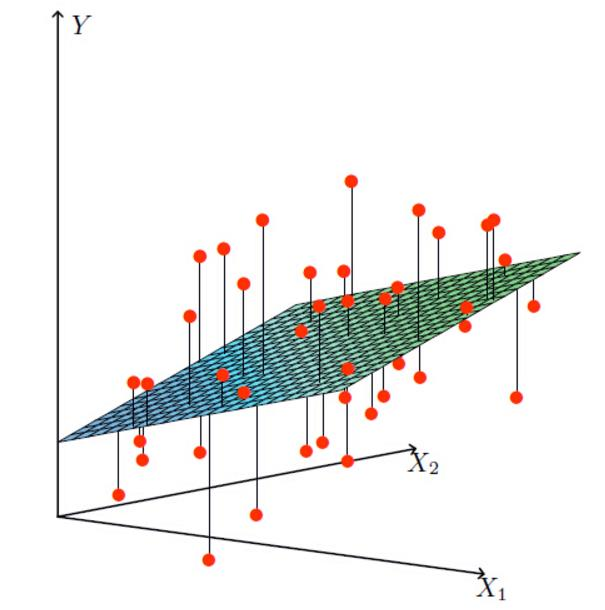
\includegraphics[scale=0.5]{fitting_plane.jpg}
		\renewcommand{\figurename}{Fig} % set picture title starting with Fig or 图
		\caption{fitting plane in sample space}
		\label{fig:1}
	\end{figure}
	the common condition is as section one show, dataset D has d property. at present, it should try to study 
	\begin{equation}f(\boldsymbol x_i) = \boldsymbol{w^{T}}\boldsymbol{x_{i}} + b\end{equation}
	\qquad let \begin{equation}f(\boldsymbol x_i)\cong{y_i}\end{equation}
	\qquad this condition named multivariate linear regression.
	\subsection{\quad analysis}
	similarly, estimate w and b by least square method. 
	conveniently, 
	\begin{equation}\hat{\boldsymbol{w}} = (\boldsymbol{w}; b)\end{equation}
	dataset D show as a matrix $\boldsymbol{X}$, shape $m\times (d+1)$
	\begin{equation}
	\boldsymbol{X}\text{=}
	\left( 
	\begin{matrix}
	{{x}_{11}} & {{x}_{12}} & \cdots  & {{x}_{1d}} & 1  \\
	{{x}_{21}} & {{x}_{22}} & \cdots  & {{x}_{2d}} & 1  \\
	\vdots  & \vdots  & \ddots  & \vdots  & \vdots   \\
	{{x}_{m1}} & {{x}_{m2}} & \cdots  & {{x}_{md}} & 1  \\
	\end{matrix} 
	\right)
	=
	\left( 
	\begin{matrix}
	x_{1}^{T} & 1  \\
	x_{2}^{T} & 1  \\
	\vdots  & \vdots   \\
	x_{m}^{T} & 1  \\
	\end{matrix} 
	\right)
	\end{equation}
	\begin{equation}\text{tag }\boldsymbol{y} = (y_1; y_2; \cdots; y_m)\end{equation}
	so fitting plane \begin{equation}h_w(x) = w_0+w_1x+w_2x+...+w_dx, w_0 
	\text{ is bias}\end{equation}
	
	in summary, \begin{equation}h_w(x) = \sum_{i=0}^{n}w_{i}x_{i} = w^{T}x\end{equation}
	
	\subsection{\quad processing}
	$\boldsymbol \varepsilon$ error, represent the difference between true and predict value.
	
	for every sample, \begin{equation}y^i = w^Tx^i + \varepsilon^i\end{equation}
	\qquad whether $\varepsilon$ obey the independent and identical distribution, and observe mean 0 and var $\theta^2$ distribution.
	
	$\varepsilon$ obey gause distribution, \begin{equation}p(\varepsilon^i) = \frac{1}{\surd{2\pi \sigma}}e\text{x}p(-\frac{(\varepsilon^i)^2}{2\sigma^2})\end{equation}
	substitution equation 16 into equation 17, as following:
	\begin{equation}
	p(y^i|x^i; w) = \frac{1}{\surd{2\pi} \sigma}e\text{x}p(-\frac{(y^i - w^T x^i)^2}{2\sigma^2})
	\end{equation}
	
	likelihood function: % explaintion: the probability every sample belong to real tag is more big and more better.
	\begin{equation}
	L(w) = \underset{i=1}{\overset{m}{\mathop{\prod }}} p(y^i|x^i; w) = \underset{i=1}{\overset{m}{\mathop{\prod }}} \frac{1}{\surd{2\pi} \sigma}e\text{x}p(-\frac{(y^i - w^T x^i)^2}{2\sigma^2})
	\end{equation}
	 
	logarithmic likelihood function: % explaintion: simplify the calculate
	\begin{equation}
		\log{L(w)} = \log{\underset{i=1}{\overset{m}{\mathop{\prod }}} p(y^i|x^i; w) = \underset{i=1}{\overset{m}{\mathop{\prod }}} \frac{1}{\surd{2\pi} \sigma}e\text{x}p(-\frac{(y^i - w^T x^i)^2}{2\sigma^2})}
	\end{equation}
	
	expand equation 20th: 
	% split could show only one tag
	\begin{align}
	\begin{split}
	L(w) &= \sum_{i=1}^{m} \log \frac{1}{\surd{2\pi} \sigma}e\text{x}p(-\frac{(y^i - w^T x^i)^2}{2\sigma^2}) \\
		 &= m\log \frac{1}{\surd{2\pi} \sigma} - \frac{1}{\sigma^2}\cdot \frac{1}{2}\sum_{i=1}^{m}(y^i - w^T x^i)^2
	\end{split}
	\end{align}
	
	target: $L(w)$ more big and more better
	\begin{equation}
	J(w) = \frac{1}{2}\sum_{i=1}^{m}(y^i - w^T x^i)^2\quad\text{(least square method)}
	\end{equation}
	
	target function:
	\begin{align}
		\begin{split}
	J(w) &= \frac{1}{2}\sum_{i=1}^{m}(h_w(x^i) - y^i)^2\\
		 &= \frac{1}{2}(\boldsymbol{X\hat{w}} - \boldsymbol{y})^T(\boldsymbol{X\hat{w}} - \boldsymbol{y})
		 \end{split}
	\end{align}
	
	solve partial derivation:
	\begin{align}
	\begin{split}
    \bigtriangledown_wJ(w) &= \bigtriangledown_w(\frac{1}{2}(\boldsymbol{X\hat{w}} - \boldsymbol{y})^T(\boldsymbol{X\hat{w}} - \boldsymbol{y}))\\
    &= \bigtriangledown_w(\frac{1}{2}(\boldsymbol{\hat{w}^TX^T} - \boldsymbol{y^T})(\boldsymbol{X\hat{w}} - \boldsymbol{y}))\\
    &= \bigtriangledown_w((\frac{1}{2}(\boldsymbol{\hat{w}^TX^TXw} - \boldsymbol{\hat{w}^TX^Ty} - \boldsymbol{yX\hat{w}} + \boldsymbol{y^Ty)})\\
    % matrix derivation
    &= \frac{1}{2}(2\boldsymbol{X^TX\hat{w}} - \boldsymbol{X^Ty} -\boldsymbol{X^Ty})\\
    &= \boldsymbol{X^TX\hat{w}} - \boldsymbol{X^Ty}
	\end{split}
	\end{align}
	
	let partial derivation be equal to 0:
	\begin{equation}
	\boldsymbol{\hat{w}} = \boldsymbol{(X^TX)^{-1}X^Ty}
	\end{equation} 
	
	estimate method:
	original estimate part 
	\begin{equation}
	R^2 = 1-\frac{\sum_{i=1}^{m}(\hat{y}_i - y_i)^2}{\sum_{i=1}^{m}(y_i - \bar{y}_i)^2}
	\end{equation}
	when $R^2$ value is very close approximation to 1, the model fits dataset D well.
	
	\subsection{\quad deep analysis}
	if $X^TX$ is irreversible or avoid over fitting, increase $\lambda$ destabilization
	\begin{equation}
	\theta = (X^TX + \lambda I)^{-1}X^Ty
	\end{equation} 
	
	to remember conclusion simply,
	\begin{align}
		\begin{split}
		X\theta = y \Rightarrow X^TX\theta = X^Ty \Rightarrow \theta = (X^TX)^{-1}X^Ty
		\end{split}
	\end{align}
	
	after add $\lambda$ destabilization:
	\begin{itemize}
		\item $X^TX$ is positive semidefinite matrix: for any non-zero vector u
		\begin{equation}
			\theta X^T X \theta = (X \theta)^T X \theta \overset{define\  v = X \theta}{  \longrightarrow} v^T v \geq 0
		\end{equation}
		\item for any real $\lambda > 0$, $X^T X + \lambda I$ is positive definite matrix, and is reversible. be sure that regerssion equation must be significative.
		\begin{equation}\theta = (X^T X + \lambda I)^{-1} X^T y\end{equation}
	\end{itemize}

	\subsection{\quad penalty factor}
	\begin{itemize}
		\item the target function of linear regerssion:
			\begin{align}
			J(\theta) = \frac{1}{2}\sum_{i=1}^{m}(h_\theta(x^i) - y^i)^2
			\end{align}
		
		\item increase square sum loss:
			\begin{align}
			J(\theta) = \frac{1}{2}\sum_{i=1}^{m}(h_\theta(x^i) - y^i)^2 + \lambda \sum_{j=1}^{m}\theta_{j}^{2}
			\end{align}
			
		\item actually, assume that parameter $\theta$ obey Gaussian distribution
	\end{itemize}

	\subsection{\quad |w|and $|\text{w}|^2$}
	\begin{figure}[H]
		\vspace{-0.2cm}  %调整图片与上文的垂直距离
		\setlength{\abovecaptionskip}{-0.2cm}   %调整图片标题与图距离
		%\setlength{\belowcaptionskip}{0.5cm}   %调整图片标题与下文距离
		\centering
		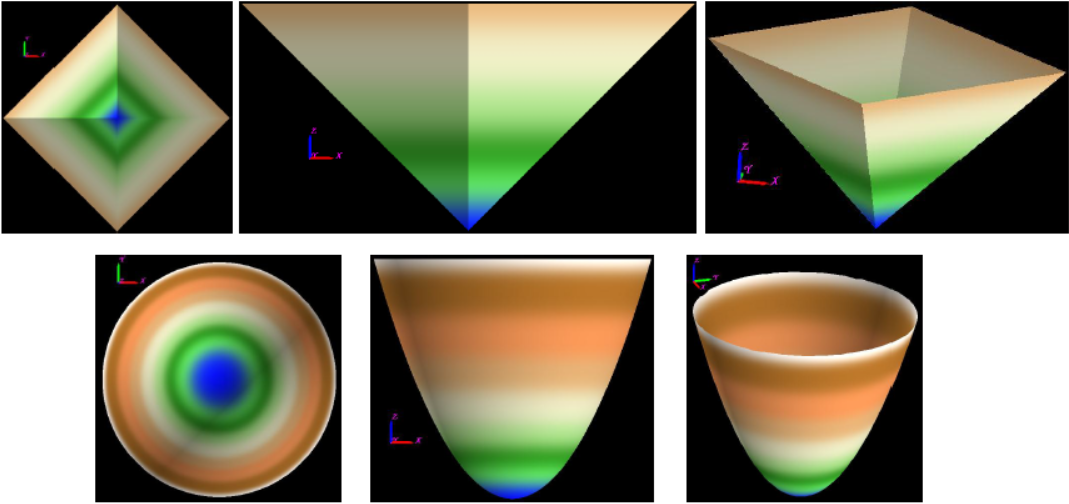
\includegraphics[scale=0.4]{w_and_w^2.png}
		\renewcommand{\figurename}{Fig} % set picture title starting with Fig or 图
		\caption{|w| and $|\text{w}|^2$}
		\label{fig:1}
	\end{figure}
		
	\section{\quad machine learning and data analysis}
	\begin{figure}[H]
		\vspace{-0.5cm}  %调整图片与上文的垂直距离
		\setlength{\abovecaptionskip}{-0.2cm}   %调整图片标题与图距离
		%\setlength{\belowcaptionskip}{-1cm}   %调整图片标题与下文距离
		\centering
		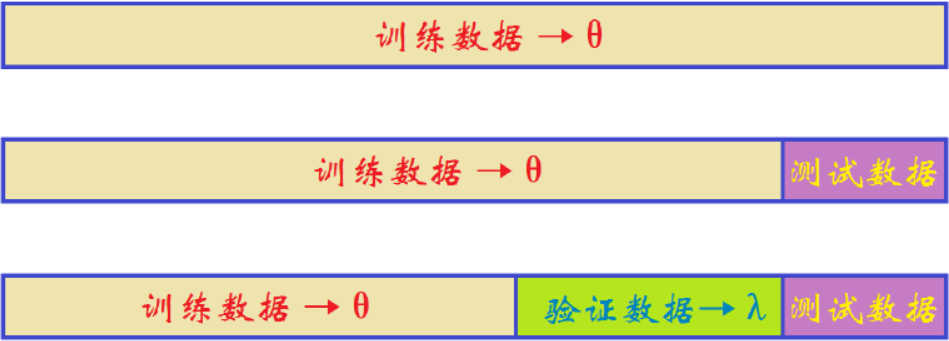
\includegraphics[scale=0.4]{machine_learning_and_data_analysis.png}
		\renewcommand{\figurename}{Fig} % set picture title starting with Fig or 图
		\caption{machine learning and data analysis}
		\label{fig:1}
	\end{figure}
	\begin{itemize}
		\item cross validation:
		\subitem example: 10 folk cross validation
	\end{itemize}
\end{document}

